\documentclass[a4paper,11pt,titlepage]{scrbook}
\usepackage[utf8]{inputenc}     
\usepackage[EU2]{fontenc} %mymurks: lualatex
\usepackage{shellesc}
                                
\usepackage{lmodern}
\usepackage[protrusion=true,expansion,tracking]{microtype}
\microtypecontext{spacing=nonfrench}
\usepackage[english,ngerman]{babel}
\usepackage[backend=biber,style=ieee]{biblatex}
\addbibresource{lit.bib}
\usepackage{amsmath}
\usepackage{amssymb}
\usepackage{mathtools}
%\usepackage{bbm}
\usepackage{upgreek}
\usepackage{nicefrac}
\usepackage[load-configurations=abbreviations]{siunitx}
\sisetup{per-mode=fraction}
\sisetup{separate-uncertainty=true}
\usepackage[version=3]{mhchem}
\usepackage{vmargin}
\usepackage{fancyhdr}
\usepackage{placeins}

\let\Oldsection\section
\renewcommand{\section}{\FloatBarrier\Oldsection}
\let\Oldsubsection\subsection
\renewcommand{\subsection}{\FloatBarrier\Oldsubsection}
\let\Oldsubsubsection\subsubsection
\renewcommand{\subsubsection}{\FloatBarrier\Oldsubsubsection}

\usepackage[nottoc,notlot,notlof]{tocbibind}
\usepackage{varioref}
\usepackage{booktabs}
\usepackage[table]{xcolor}
\definecolor{kitcolor}{rgb}{0 0.61 0.50}
\usepackage[pdftex]{graphicx}
\usepackage[normal,font={small,color=black},labelfont=bf,margin=2em]{caption}
\usepackage{subfig}
\usepackage[absolute,overlay]{textpos}
\usepackage{tikz}
\usetikzlibrary{external}
\tikzexternalize[optimize=false,prefix=tikz/]
\usepackage{ifthen}
\usepackage[fit,breakall]{truncate}
\usepackage{etoolbox}
\usepackage{xstring}
\usepackage{multicol}
\DeclareGraphicsRule{*}{mps}{*}{}
\DeclareGraphicsExtensions{.eps,.pdf,.png,.jpg,.jpeg,.mps}
\usepackage{epstopdf}
\usepackage[raiselinks=true,bookmarks=true, bookmarksopenlevel=1,bookmarksopen=true,bookmarksnumbered=true,hyperindex=true,plainpages=false,pdfpagelabels=true,pdfborder={0 0 0.5},colorlinks=false,linkbordercolor=kitcolor,citebordercolor=kitcolor]{hyperref}
%% -----------------------
%% |    Abbreviations    |
%% -----------------------
\newcommand{\op}[1]{\operatorname{#1}}                 % to write operators that
                                                       % are not predefined;
                                                       % it's just an abbrev.
                                                       % for the long command

\newcommand{\arr}[2]{\begin{array}{#1}#2\end{array}}   % to create arrays. very 
                                                       % useful in math env

\renewcommand{\d}{\ensuremath{\text{d}}}               % as the differential 
                                                       % operator, e.g. 
                                                       % \frac{\d x}{\d t}

\newcommand{\NN}{\mathbb{N}}                           % or change it to
\newcommand{\RR}{\mathbb{R}}                           % \mathbbm and include
\newcommand{\CC}{\mathbb{C}}                           % pkg bbm if you prefer

\newcommand{\pdb}[2]{\frac{\partial #1}{\partial #2}}  % partial derivative


%% -----------------------------------
%% |    Commands and Environments    |
%% -----------------------------------
\newcommand{\margtodo}                                 % used by \todo command
{\marginpar{\textbf{\textcolor{kitcolor}{ToDo}}}{}}
\newcommand{\todo}[1]
{{\textbf{\textcolor{kitcolor}{[\margtodo{}#1]}}}{}}   % for todo-notes inside 
                                                       % the document
\newenvironment{deprecated}                            % for something that you
{\begin{color}{gray}}{\end{color}}                     % want to use no more

\newcommand{\xcaption}[2]{\caption[#1]{\textbf{#1} #2}}% nice caption cmd for
                                                       % short and long descrip.

\newcommand{\xfigure}[5]{\begin{figure}[#1]            % a quick command for
\centering                                             % including graphics 
\includegraphics[scale=#2]{./fig/#3}                   % with all necessary vars
\xcaption{#4}{#5}
\label{fig:#3}
\end{figure}}

\newcommand{\xfigurerot}[5]{\begin{figure}[#1]        % same as above, only
\centering                                            % image is rotated
\includegraphics[angle=270,scale=#2]{./fig/#3}
\xcaption{#4}{#5}
\label{fig:#3}
\end{figure}}

\newcommand{\xtable}[4]{\begin{table}[#1]             % same for tables
\centering
\xcaption{#3}{#4}
\rowcolors{3}{gray!10}{white}
\include{./tab/#2}
\label{tab:#2}
\end{table}}



%% ------------------------------------
%% |    Quantum Mechanics and Math    |
%% ------------------------------------
\newcommand{\ket}[1]{\left|#1\right\rangle}           % \ket{X}  ->  |X>
\newcommand{\bra}[1]{\left\langle#1\right|}           % \bra{X}  ->  <X|
\newcommand{\braket}[2]                               % \braket{X}{Y}  ->  <X|Y>
{\left\langle#1 \middle| #2\right\rangle}
\newcommand{\bratenket}[3]                            % \bratenket{X}{Y}{Z}  ->
{\left\langle#1 \middle|\middle| #2 \middle|\middle|  % <X|Y|Z>
#3\right\rangle}
\newcommand{\anglemean}[1]                            % \anglemean{X}  ->  <X>
{\left\langle #1 \right\rangle}                       % \norm{X}  ->  || X ||
\newcommand{\norm}[1]{\left\lVert#1\right\rVert}

\newcommand{\updownarrows}                            % \ket\updownarrows  ->
{\text{\rotatebox[origin=c]{90}{$\rightleftarrows$}}} % |↑↓> (cmt is utf8!)
\newcommand{\downuparrows}                            % \ket\updownarrows  ->
{\text{\rotatebox[origin=c]{270}{$\rightleftarrows$}}}% |↓↑>
\newcommand{\neswarrows}                              % \ket\neswarrows  ->
{\text{\rotatebox[origin=c]{45}{$\rightleftarrows$}}} % |↗↙>
\newcommand{\swnearrows}                              % \ket\swnearrows  ->
{\text{\rotatebox[origin=c]{225}{$\rightleftarrows$}}}% |↙↗>

\newcommand{\cre}{c^\dagger}                          % annihalation operator
\newcommand{\anh}{c^{\vphantom{\dagger}}}             % creation operator
\newcommand{\numb}{n^{\vphantom{\dagger}}}            % number operator

\newcommand{\fullstop}{\text{\,.}}                    % fullstop or comma in
\newcommand{\comma}{\text{\,,}}                       % math mode for use
                                                      % after equations
                                                      
                                                      

\setcounter{secnumdepth}{3}           % Numbering also for \subsubsections
\setcounter{tocdepth}{3}              % Register \subsubsections in content dir

\setpapersize{A4}
\setmarginsrb{3cm}{1cm}{3cm}{1cm}     % {leftmargin}{topmargin}{rightmargin}...
             {6mm}{7mm}{5mm}{15mm}    % {bottommargin}{headheight}{headsep}...
                                      % {footheight}{footskip}

\setlength{\marginparwidth}{1.5cm}    % for todos to be positioned correctly

\parindent 0cm                        % do not indent beginning of paragraph
\parskip 1.5ex plus0.5ex minus0.5ex   % Margin between paragraphs





%% ------------------------
%% |    Language Setup    |
%% ------------------------
\newcommand{\SelectLanguage}[1]
{
    \AtBeginDocument
    {
        \selectlanguage{#1}           % babel command

        \iflanguage{ngerman}
        {
            \sisetup{output-decimal-marker={,}}
            % sets , for German and . otherwise
            \sisetup{list-final-separator={ und }}
            % "3, 4 and 5" in English or "3, 4 und 5" in German
            \sisetup{range-phrase={ bis }}
            % "1.5 to 1.8" in English or "1,5 bis 1,8" in German
            \sisetup{locale=DE}
            % e.g. using \cdot instead of \times for floating points
        }
        {
            \sisetup{output-decimal-marker=.}
            \sisetup{list-final-separator={ and }}
            \sisetup{range-phrase={ to }}
        }
    }
}





%% ---------------------------
%% |    Style of captions    |
%% ---------------------------
\newcommand{\changefont}[3]{\fontfamily{#1} \fontseries{#2}%
                            \fontshape{#3} \selectfont}
\newcommand{\chapterheadfont}{}

\renewcommand{\chaptername}{}

\makeatletter
\renewcommand{\section}{%
\@startsection{section}%
{1}                                    % Structure level
{0mm}                                  % Indention
{2ex plus 1ex minus 1ex}               % Pre-Margin
{0.5ex plus 0.5ex minus 0.5ex}         % Post-Margin
{\chapterheadfont\large\bfseries}      % Style
}
\renewcommand{\subsection}{%
\@startsection{subsection}%
{2}                                    % Structure level
{0mm}                                  % Indention
{1.5ex plus 1ex minus 0.5ex}           % Pre-Margin
{0.3ex plus 0.3ex minus 0.3ex}         % Post-Margin
{\chapterheadfont\large\bfseries}      % Style
}
\renewcommand{\subsubsection}{%
\@startsection{subsubsection}%
{3}                                    % Structure level
{0mm}                                  % Indention
{1.5ex plus 1ex minus 0.5ex}           % Pre-Margin
{0.2ex plus 0.2ex minus 0.2ex}         % Post-Margin
{\chapterheadfont\normalsize\bfseries} % Style
}
\renewcommand{\paragraph}{%
\@startsection{paragraph}%
{4}                                    % Structure level
{0mm}                                  % Indention
{1.3ex plus 1ex minus 0.3ex}           % Pre-Margin
{0.2ex plus 0.2ex minus 0.2ex}         % Post-Margin
{\chapterheadfont\normalsize\bfseries} % Style
}
\renewcommand{\subparagraph}{%
\@startsection{subparagraph}%
{5}                                    % Structure level
{0mm}                                  % Indention
{1ex plus 1ex minus 0.2ex}             % Pre-Margin
{0.1ex plus 0.1ex minus 0.1ex}         % Post-Margin
{\chapterheadfont\normalsize\bfseries} % Style
}
\makeatother




%% -----------------------------------
%% |    Style of chapter captions    |
%% -----------------------------------
\newlength{\chapnolen}
\newlength{\chapparlen}
\newsavebox{\chapno}
\makeatletter
\renewcommand{\@makechapterhead}[1]{
    \vspace*{0.1\textheight}
    \vskip 15\p@
    {\parindent \z@ \raggedright \normalfont
        \ifnum \c@secnumdepth >\m@ne
            \if@mainmatter
                \savebox{\chapno}{\chapterheadfont\huge\bfseries \thechapter.}
                \settowidth{\chapnolen}{\usebox{\chapno}}
                \parbox[t]{\chapnolen}{\usebox{\chapno}}\nobreak\leavevmode
            \fi
        \fi
        \interlinepenalty\@MM
        \setlength{\chapparlen}{\textwidth}
        \addtolength{\chapparlen}{-1.0\chapnolen}
        \addtolength{\chapparlen}{-2ex}
        \leavevmode\nobreak
        \parbox[t]{\chapparlen}%
        {\raggedright\chapterheadfont\huge \bfseries #1\par\nobreak}
        \vskip 30\p@
    }}


\renewcommand{\@makeschapterhead}[1]{
    \vspace*{50\p@}
    {\parindent \z@ \raggedright
        \normalfont
        \interlinepenalty\@M
        \chapterheadfont \huge \bfseries  #1\par\nobreak
        \vskip 40\p@
    }
}





%% ------------------------------------
%% |    Style of content directory    |
%% ------------------------------------
\let\oldtableofcontents\tableofcontents
\renewcommand{\tableofcontents}{{\pdfbookmark{\contentsname}{\contentsname}%
\chapterheadfont\oldtableofcontents}}
\let\@olddottedtocline\@dottedtocline
\renewcommand{\@dottedtocline}[5]{\@olddottedtocline{#1}{#2}{#3}{#4}%
{\chapterheadfont #5}}
\makeatother




%% ------------------------------------------
%% |    Style of appendix and mainmatter    |
%% ------------------------------------------
\newcommand{\FrontMatter}
{
    \frontmatter

    \pagestyle{empty}

    \fancypagestyle{plain}{            % to ensure toc page style is really 
                                       % empty (it uses \thispagestyle{plain})
        \fancyhf{}                     % clear all header and footer fields
        \fancyfoot{}                   % except the center
        \renewcommand{\headrulewidth}{0pt}
        \renewcommand{\footrulewidth}{0pt}
    }
}

\newcommand{\MainMatter}
{
    \clearpage

    \begingroup                        % make sure that there is no involuntary 
                                       % blankpage added after toc.
    \let\cleardoubleoddstandardpage\relax
    \mainmatter
    \endgroup

    \frontmatter \pagestyle{empty}

    \fancypagestyle{plain}{            % redefine chapter first page style,
                                       % which is redefined by \FrontMatter
        \fancyhf{}                     % clear all header and footer fields
        \fancyfoot[C]{\thepage}        % except the center
        \renewcommand{\headrulewidth}{0pt}
        \renewcommand{\footrulewidth}{0pt}
    }

    \mainmatter
    \pagestyle{fancy}
    \renewcommand{\chaptermark}[1]{\markboth{\chaptername\ %
                                             \thechapter.\ ##1}{}}
    \lhead[\thepage]{\leftmark}\chead[]{}\rhead[\thesispagehead]{\thepage}
    \lfoot{}\cfoot{}\rfoot{}
}

\newcommand{\Appendix}
{
    \clearpage
    \appendix
    \setcounter{section}{0}
    \setcounter{subsection}{0}
    \setcounter{figure}{0}
    \setcounter{equation}{0}
    \renewcommand\thesection{\Alph{section}}
    \renewcommand\thefigure{\Alph{section}.\arabic{figure}}
    \renewcommand\thetable{\Alph{section}.\arabic{table}}
    \renewcommand\theequation{\Alph{section}.\arabic{equation}}
    \numberwithin{equation}{section}
    \lhead[\thepage]{Appendix}
}

\newcommand{\TheBibliography}
{
    \clearpage
    \thispagestyle{plain}
}

\newcommand{\emptychapter}[2][]
{
    \addtocounter{chapter}{1}
    \addtocontents{toc}{\protect\contentsline
        {chapter}{\protect\numberline {\thechapter}#2}{#1}{}}
}


%mystuff
%floatbarriers also for subsections
%https://tex.stackexchange.com/questions/118662/use-placeins-for-subsections
\makeatletter
\AtBeginDocument{%
  \expandafter\renewcommand\expandafter\subsection\expandafter{%
    \expandafter\@fb@secFB\subsection
  }%
}
\makeatother


%myinputs
\usepackage{hyperref}
\usepackage{amsmath}
\usepackage{siunitx}
\usepackage{float}
\usepackage{tabularx}
\usepackage{pgfplots}
\pgfplotsset{compat=newest}
\usepackage{tikzscale}


\usetikzlibrary{shapes,arrows.meta}
\usepackage{listings}
\lstset{
  literate={ö}{{\"o}}1
           {ä}{{\"a}}1
           {ü}{{\"u}}1
           {Ü}{{\"U}}1
           {Ö}{{\"O}}1
           {Ä}{{\"A}}1
}
\definecolor{mygreen}{RGB}{28,172,0} % color values Red, Green, Blue
\definecolor{mylilas}{RGB}{170,55,241}

\lstdefinelanguage{AHDL}
{
	% list of keywords
	morekeywords={
		import,
		if,
		then,
		while,
		for,
		table,
		variable,
		subdesign,
		signal,
		machine,
		of,
		bits,
		with,
		states,
		begin,
		end
	},
	sensitive=false, % keywords are not case-sensitive
	morecomment=[l]{\%} % l is for line comment
	tabsize=2
}

%common settings
%\lstset{
%    breaklines=true,%
%    morekeywords={},
%    keywordstyle=\color{blue},%
%    morekeywords=[2]{1}, keywordstyle=[2]{\color{black}},
%    identifierstyle=\color{black},%
%    stringstyle=\color{mylilas},
%    commentstyle=\color{mygreen},%
%    showstringspaces=false,%without this there will be a symbol in the places where there is a space
%    numbers=left,%
%    numberstyle={\tiny \color{black}},% size of the numbers
%    numbersep=9pt, % this defines how far the numbers are from the text
%    tabsize=2,
%    basicstyle=\footnotesize\ttfamily
%}

%prevent copying line numbers over from pdf
\usepackage{accsupp}
\newcommand{\noncopynumber}[1]{%
    \BeginAccSupp{method=escape,ActualText={}}%
    #1%
    \EndAccSupp{}%
}
%common settings
\lstset{columns=flexible}
\lstset{keepspaces=false}
\lstset{
    breaklines=true,%
    morekeywords={},%
    frame=tb,
    basicstyle={\footnotesize},
    keywordstyle=\bfseries,%
    showstringspaces=false,%without this there will be a symbol in the places where there is a space
    numbers=left,%
    numberstyle=\tiny\noncopynumber,% size of the numbers
    numbersep=9pt, % this defines how far the numbers are from the text
    tabsize=2%  
}


\lstdefinestyle{vhdl}
{
    language=VHDL,%
}

\lstdefinestyle{ahdl}
{
    language=AHDL,%
}

\lstdefinestyle{verilog}
{
    language=Verilog,%
}

\lstdefinestyle{python}
{
    language=Python,%
}






\SelectLanguage{english}
\newcommand{\thesisauthor}{Marvin-Dennis Noll}
\newcommand{\thesistopic}{Stability Improvements at FLUTE}
\newcommand{\thesisentopic}{Verbesserung der Stabilität von FLUTE}
\newcommand{\thesislongtopic}{}
\newcommand{\thesisinstitute}{Institute for Beam Physics and Technology}
\newcommand{\thesisreviewerone}{Prof. Dr.-Ing. John Jelonnek (IHM)}
\newcommand{\thesisreviewertwo}{Prof. Dr. Anke-Susanne Müller (IBPT)}
\newcommand{\thesisadvisorone}{Dr. Nigel Smale (IBPT)} % to use: enter names and uncomment in titlepg
\newcommand{\thesisadvisortwo}{}
\newcommand{\thesistimestart}{15.11.2020} % on titlepage
\newcommand{\thesistimeend}{01.07.2021} % on titlepage
\newcommand{\thesistimehandin}{01.07.2021} % on second page 'preamble'
\newcommand{\thesispagehead}{Master Thesis: \thesisentopic} % page heading

\hypersetup
{
    pdfauthor={\thesisauthor},
    pdftitle={Masterarbeit: \thesistopic},
    pdfsubject={\thesislongtopic},
    pdfkeywords={kit,physics,master,thesis,\thesisauthor}
}

\begin{document}
    % Titlepage and ToC
    \FrontMatter

    \tikzexternaldisable
% coordinates for background border
\newcommand{\diameter}{20}
\newcommand{\xone}{-15}
\newcommand{\xtwo}{160}
\newcommand{\yone}{15}
\newcommand{\ytwo}{-253}




\begin{titlepage}
    % background border
    \begin{tikzpicture}[overlay]
    \draw[color=gray]
            (\xone mm, \yone mm)
      -- (\xtwo mm, \yone mm)
    arc (90:0:\diameter pt)
      -- (\xtwo mm + \diameter pt , \ytwo mm)
        -- (\xone mm + \diameter pt , \ytwo mm)
    arc (270:180:\diameter pt)
        -- (\xone mm, \yone mm);
    \end{tikzpicture}



    % KIT image and sign for faculty of physics
    \begin{textblock}{10}[0,0](4.5,2.5)
        \includegraphics[width=.25\textwidth]{include/kitlogo.pdf}
    \end{textblock}
    \changefont{phv}{m}{n}    % helvetica
    \begin{textblock}{10}[0,0](5.5,2.2)
        \begin{flushright}
            \Large DEPARTMENT OF PHYSICS\\\thesisinstitute
        \end{flushright}
    \end{textblock}



    % horizontal line
    \begin{textblock}{10}[0,0](4.2,3.1)
        \begin{tikzpicture}[overlay]
        \draw[color=gray]
                (\xone mm + 5 mm, -12 mm)
          -- (\xtwo mm + \diameter pt - 5 mm, -12 mm);
        \end{tikzpicture}
    \end{textblock}



    % begin of text part
    \changefont{phv}{m}{n}    % helvetica
    \centering



    % thesis topic (en and ge)
    \vspace*{3cm}
    \Huge\thesistopic\\
    \huge(\thesisentopic)\\



    % author name and institute
    \vspace*{2cm}
    \Large Master thesis\\of\\
    \vspace*{1cm}
    \huge\thesisauthor\\
    \vspace*{1cm}
    \Large at the \thesisinstitute



    % possible frontimage - thanks to JabberWok
    % for publishing the img under GNU Document License
    \vspace*{6.5cm}
    %\includegraphics[scale=0.7]{./include/frontimage.eps}\\



    % examiners (Referenten)
    \vspace*{1.5cm}
    \Large
    \begin{center}
        \begin{tabular}[ht]{l c l}
        \iflanguage{english}{Reviewer}{Referent}: 
            & \hfill & \thesisreviewerone\\
        \iflanguage{english}{Second Reviewer}{Korreferent}: 
            & \hfill & \thesisreviewertwo\\
        % uncomment if you want to provide info on your advisors
        \iflanguage{english}{Advisor}{Betreuender Mitarbeiter}: 
            & \hfill & \thesisadvisorone\\
        %\iflanguage{english}{Second Advisor}{Zweiter betreuender Mitarbeiter}: 
        %    & \hfill & \thesisadvisortwo\\
        \end{tabular}
    \end{center}



    % working time
    \vspace{1cm}
    \begin{center}
        \large{\thesistimestart \hspace*{0.25cm} -- %
                                   \hspace*{0.25cm} \thesistimeend}
    \end{center}



    % lowest text blocks concerning the KIT
    \begin{textblock}{10}[0,0](2,16.8)
        \tiny{KIT – The Research University in the Helmholtz Association}
    \end{textblock}
    \begin{textblock}{10}[0,0](10,16.75)
        \large{\textbf{www.kit.edu}}
    \end{textblock}
\end{titlepage}
\tikzexternalize[optimize=false,prefix=tikz/]

    \chapter*{Erklärung zur Selbstständigkeit}
Ich versichere wahrheitsgemäß, die Arbeit selbstständig angefertigt, alle benutzten Hilfsmittel vollständig und genau angegeben und alles kenntlich gemacht zu haben, was aus Arbeiten anderer unverändert oder mit Abänderungen entnommen wurde und dass ich die Satzung des KIT zur Sicherung guter wissenschaftlicher Praxis in der gültigen Fassung vom 24.05.2018 beachtet habe.\\

\vspace{1cm}

\renewcommand{\arraystretch}{0} % for spacing in the tabular environment

\begin{flushright}
	\begin{tabular}{rr}
		Karlsruhe, den \thesistimehandin, & \hspace*{5cm}\\[0mm]
		\cline{2-2}\\[2mm]    % the last line has height 2mm due
		& \thesisauthor       % to \arraystretch=0
	\end{tabular}
\end{flushright}

\vfill

\begin{flushright}
	Als Prüfungsexemplar genehmigt von\\
	\vspace{1cm}
	\begin{tabular}{rr}
		Karlsruhe, den \thesistimehandin, & \hspace*{5cm}\\[0mm]
		\cline{2-2}\\[2mm]    % the last line has height 2mm due
		& \thesisreviewerone  % to \arraystretch=0
	\end{tabular}
\end{flushright}

\renewcommand{\arraystretch}{1}

\cleardoublepage


    \begingroup \let\clearpage\relax    % in order to avoid listoffigures and
    \tableofcontents                    % listoftables on new pages
    \listoffigures
    \listoftables
    \endgroup
    \cleardoublepage

    % Contents
    \MainMatter

	%\chapter*{Abstract}
\gls{flute}, a compact linear accelerator, is currently designed and under commission at \gls{kit}. Its main purposes are to serve as a technology platform for accelerator research, the generation of strong and ultra short \gls{thz} pulses and in the future as an injection device for the \gls{cstart}.

At the current commissioning state, the klystron which powers the microwave cavity in the electron gun and, in later stages, the linear accelerator is fed by a pulse forming network, which is driven by a high voltage source connected to mains power. To ensure stable energies of the emitted electron bunches, several parameters of the cavity, such as temperature, as well as the power supply, such as \gls{rf} power, have to stay inside tight tolerance bands.

In the past, a predominant source of instability were slow drifts of the \gls{rf} power due to interference with the \SI{50}{\hertz} of the mains voltage. After dealing with this issue, the cavity \gls{rf} power stability was improved significantly, which also improves the electron stability. But further improvements to the stability are still desired to make the whole system usable for scientific experiments, such as \gls{thz} spectroscopy.

In this work, instead of passively optimizing the stability of system components, an active approach is evaluated. By means of a control system, the amplitude of the low power \gls{rf} input signal of klystron, the effects of noise and/or drifts shall be mitigated.

As part of the development process, first the stability issue is analyzed and metrics for the stability are defined. Then the solution, a control system, is proposed. After that, the necessary building blocks of such a control system are treated in detail. From an evaluation of the sensors and actuators, the controller is designed and its positive effect on the gun stability is verified both by simulation and on the actual \gls{flute} accelerator. In both cases a considerable improvement is noticeable. 

\cleardoublepage

	%\chapter{Introduction}
In this thesis methods to improve the stability of the electron gun of the \gls{flute} accelerator are studied.

\Gls{flute} is a \gls{thz} photon source based on a \gls{linac} and is currently under commission at the \gls{kit}. It aims to be a source of high field \gls{thz} pulses (up to \SI{1200}{\mega\volt\per\meter}) in the femtosecond range, provide a test facility for accelerator research and an injection device for \gls{cstart} (see \cite{SchaeferHaererPapash2019_1000091183}) in the future. \cite{Naknaimueang:2011zz}

The accelerator is designed for a final electron momentum of \SI{41}{\MeV\per c} and bunch charges of \SIrange{1}{3000}{\pico\coulomb} with lengths of \SIrange{1}{300}{\fs}. The bunches are emitted with a repetition frequency of up to \SI{10}{\hertz}. \cite{Malygin2018}

\autoref{fig:fluteEgun-flutePaper} shows the finished accelerator schematically. Is mainly consists of the low energy section, the \gls{linac}, the four-dipole bunch compressor and several diagnostic instruments.\\
Along with several diagnostic devices, the low energy section contains the electron gun that pre-accelerates electrons to \SI{7}{\MeV\per c}. The electrons are generated at the cathode inside the gun photo-electrically through stimulation with \gls{uv} radiation (\SI{270}{\nm}) generated by a Ti:Sa laser. After that a solenoid is used to focus the electron beam for injection into the \gls{linac} section. The \gls{linac}, a 156-cell traveling wave structure, is then used to accelerate the electrons to \SI{41}{\MeV\per c}. With a setup of four dipole magnets, the bunches are compressed longitudinally before the last dipole is used to generate \gls{csr} and \gls{cer} for \gls{thz} experiments. Another way of generating \gls{thz} pulses is to use a metal target, with a specific working function, that is hit by the electron bunch. \cite{Nasse:IPAC13-WEPWA010}

At the time of writing, the low energy section is fully operational and at the end, a Faraday cup is installed as a beam dump to measure the electron bunch charges. It has to be removed when the \gls{linac} section is commissioned.

\begin{figure}[tb]
	\centering
	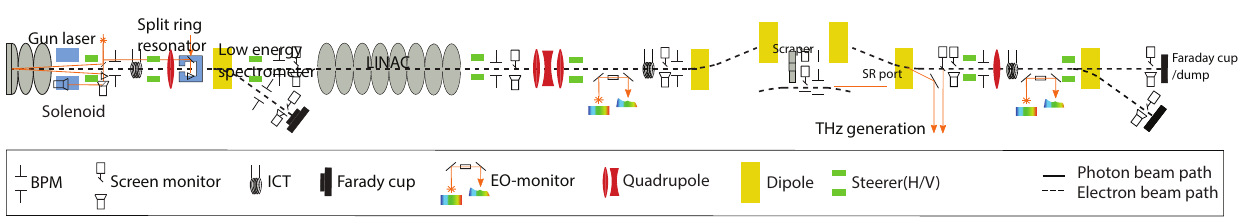
\includegraphics[width=\textwidth]{chap/StabilityOfTheElectronGun/img/flutePaper.png}
	\caption[FLUTE schematic with all components]{Schematic of the finished accelerator showing all installed and planned components (reprinted from \cite{Yan2018})}
	\label{fig:fluteEgun-flutePaper}
\end{figure}

Scientific experiments, such as \gls{thz} spectroscopy, rely on a known and stable wavelength of the \gls{thz} radiation. As the \gls{thz} radiation is emitted from a metal target by the photo effect after being hit by the electron bunches or by interaction with a magnetic field, the wavelength and the wavelength stability of the \gls{thz} photons depend on the energy and the energy stability of the electrons.
Also as \gls{flute} being a test facility, adding and changing out components, possibly developed by other research institutes, is a common routine. To ensure compatibility among these components, reliable beam parameters at the interfaces between them are necessary. These parameters include the beams position in the $x$- and $y$-direction, the beam steering angle, the electron energy, the emittance and the charge of the bunch and its dimensions. Since focusing and steering of the beam is done with electromagnets, it is also effected by the electron energy, as the deflection of an electron in a magnetic field is a function of its velocity, so ultimately its energy.

Besides depending on the wavelength of the \gls{uv} pulses hitting the cathode, the electron energies also strongly dependent of the  on the geometrical, electrical and thermal characteristics of the electron gun and its \gls{rf} power supply. These characteristics are not independent of each other and variations of them can have a multitude of intrinsic or extrinsic causes.

To improve the stability of the electron energy, in this thesis these causes are analyzed and measures against them or their effects are developed. Eventually this leads to the design of a \textit{closed}-loop control system. 

This approach is different from past efforts to improve the stability, which primarily treated the stability of (sub-) components that supply the electron gun. For instance, instabilities due to temperature variations were dealt with by stabilizing the water cooling system of the electron gun, or disturbances from the pulse forming network were reduced by improving the power supply. These measures can be thought of changes to an \textit{open}-loop. This is because there is no feeding back of the success or error from the system output, the electron energy, to the water cooler or power supply. Hence for these improvements to work, deep knowledge of the relation between the components and their effect on the electron energy is required. Also if parameters of the components change due to aging, environmental factors, such as temperature or noise on the mains power, these effects can be carried over to the electron energy.

These are the main two reasons that motivate a closed-loop approach. It is often not required to know the exact relationships between certain input disturbances and the electron energy. Most of the times qualitative descriptions or correlations are sufficient, at least as a starting point, to achieve sufficiently good rejection of the disturbances. And with a closed-loop the system can react to changes of system parameters without the need for manual modifications.

That is why in the following chapter such a closed-loop control system for the \gls{flute} electron gun is treated in detail. In order to design an appropriate control system, some prerequisites are needed. First the present disturbances are analyzed and metrics to later measure the favorable effect of the control system are defined. Then ways of connecting the finished control system to the existing hard- and software are shown. With this preliminary work done, the control system can be designed. After the design process, the whole system is simulated on a computer to verify the solution, before the control system is implemented and tested with the real hardware, i.e. at \gls{flute}.


	%\chapter{Theoretical Framework}
\section{Accelerator Physics}
\section{Signal Analysis}
\section{Feedback Control Systems}
	%\chapter{Stability of the Electron Gun}
	%\chapter{Interfacing the FLUTE RF System}
	\chapter{Controller Design and Evaluation}
In this chapter stabilizing the power output of FLUTE by means of a control system is examined. This is different than previous attempts in that a feedback control system tries to compensate short term disturbances and long term drifts \textit{actively} by interfering with some part of FLUTE that has influence of the output power.

The next sections describe the chosen architecture of a suitable control system as well as some implementation details and the tuning of necessary controller parameters.

\section{Architecture}
The general structure of a closed loop control system is shown in \autoref{fig:own-work-architecture}.

$y(t)$ is the physical quantity which should follow a certain time trajectory $x(t)$ or be kept constant (then $x(t)=x=const.$). If there are no disturbances $d(t)$ or the disturbances are deterministic (i.e. $d(t)$ is known $\forall t$), then an open loop system would be possible. In that case the role of the controller would be to merely to set its output $u(t)$ according to the system dynamics of the plant\footnote{Assuming $g(t)$ is a stable LTI system} (represented by its impulse response $g(t)$).

In most real world scenarios, $d(t)$ originates from a stochastic process and thus is unknown. Too remedy the negative influences of $d(t)$, the output $y(t)$ is measured and feed back. Based on the error $e(t)$, which is the difference between the set value and the actual value defined by
\begin{equation}
e(t) = x(t) - y(t),
\end{equation}
the controller can react accordingly.

\begin{figure}[tb]
	\centering
	\includegraphics[width=\textwidth]{chap/Controller-Design-And-Evaluation/img/controller/architecture.tikz}
	\caption{General structure of a closed loop feedback control system}
	\label{fig:own-work-architecture}
\end{figure}


\section{Inputs and Outputs}
Since the control algorithm should be implemented, tested and used online on the actual accelerator instead of only operate on simulated data, there is the need for fast and reliable interfaces to the machine.
Following, ``input'' refers to the signal going into the control algorithm (i.e. the measured $y(t)$), while ``output'' is the output of the control algorithm $u(t)$.

\subsection{Input}
Depending on which value is chosen to be controlled, filtering of the input signal could be mandatory.

In the case of the cavity RF power the signal jumps to zero each time a breakdown occurs, shortening the RF supply. These outliners are not representative of the average RF power inside the cavity over multiple pulses and thus would greatly impair the controller performance. For that reason, before any further filtering to remove noise etc, a breakdown removal filter is used (\autoref{lst:control-system-breakdownremoval}). In principle the new power value is checked to be inside a band which size is determined by the mean deviation of the $N_{filt}$ previous values and a scaling $m$. The percentile differences are used here as they are robust against outliners (i.e. other breakdowns) in the $N_{filt}$ previous values opposed to a normal standard deviation. The scaling with $(2*1.2815)^{-1}$ is used to make the mean deviation comparable to a standard deviation.

\begin{lstlisting}[style=python,caption = Breakdown removal, label = lst:control-system-breakdownremoval]
#...
if(abs(P[i]-np.median(P[i-3*Nfilt:i-Nfilt]))<
m*(np.percentile(P[i-3*Nfilt:i-Nfilt],90)-np.percentile(P[i-3*Nfilt:i-Nfilt],10)/(2*1.2815))):
   P_filt=np.append(P_filt,P[i])
else:
   breakdown_locations_predicted=np.append(breakdown_locations_predicted,i)
   P_filt=np.append(P_filt,np.median(P[i-3*Nfilt:i-Nfilt]))
#...
\end{lstlisting}




\subsection{Output}
For the control system to work the controller needs some way of influencing the plant. For that the output of the FLUTE LLRF vector modulator is controlled by a RF attenuator (see \autoref{chap:atten}).

\section{Plant Identification}
\subsection{Principle}
Before choosing an appropriate controller, some insight of the system response has to be obtained. For that reason, next the plant transfer function is obtained. In the time domain, the transfer function is the response of the system to an impulse on the input. So per definition, in the special case here, this would mean changing the RF attenuator quickly from a big attenuation to a small attenuation and then back. This is not easy to measure and a single measurement is very susceptible to noise. Therefore it is more common to measure the step response instead and to average over several step responses.

When there is no prior knowledge over the system, the identification is sometimes done with a (pseudo) random binary sequence to excite the system with step functions of different lengths. Then it is necessary that some of the steps last longer than a few dominant time constants of the system. To get the transfer function of the system from its step response, several methods are common, including correlation based and frequency response based algorithms.

\subsection{Identifying the system response of the FLUTE LLRF}
The input sequence is generated by modulating the RF attenuator around a base attenuation. As a trade off between high SNR and driving the LLRF in a ``save'' region, the control voltage span is chosen to be \SI{4}{\volt} in total (\SIrange{7}{11}{\volt} around the base control voltage of \SI{9}{\volt}).

To get a random binary sequence, depending on the outcome of a binomial random process, the voltage is toggled between \SI{7}{\volt} and \SI{11}{\volt} according to \autoref{lst:own-work-randomSequence}. With the parameter \texttt{toggleP}, the average length of one constant voltage level can be controlled.

\begin{lstlisting}[style=python,caption = Function to get a random binary sequence, label = lst:own-work-randomSequence]
def randomBinarySequence(N,toggleP):
    u=[False]*N
    for i in range(1,len(u)):
        if(np.random.binomial(1,toggleP,1)[0]):
            u[i]=not u[i-1]
        else:
            u[i]=u[i-1]
    return list(map(lambda x: 7 if x==False else 11,u))
\end{lstlisting}

In a test run over 6 hours (after FLUTE had stabilized), the attenuator was driven with such a random sequence. The result is shown in \autoref{fig:own-work-identify-input}.

\begin{figure}[tb]
	\centering
	\includegraphics[width=\textwidth,height=0.5\textwidth]{chap/Controller-Design-And-Evaluation/img/controller/time.tikz}
	\caption{Small section of the input sequence (green) and the system response (blue)}
	\label{fig:own-work-identify-input}
\end{figure}

The time signals are then split into a estimation data set (about \SI{80}{\percent} of samples) and a validation data set (the remaining $\approx$ \SI{20}{\percent}).

The two data sets are then loaded into the \textsc{Matlab} \textit{System Identification Toolbox} (SIT). With the SIT, first the means of both sets and both the input and output are removed, which is required by the estimators used. Then with different numbers of poles and zeros, the transfer function is estimated. After trying several settings, three promising candidates

\begin{align}
\hat{G}_1(s) &= \frac{71.37\,s + 0.5966}{s^3 + 0.8208\,s^2 + 0.328\,s + 0.002733} \\[1em]
\hat{G}_2(s) &= \frac{-0.2125\,s + 70.85}{s^2 + 0.8022\,s + 0.3202} \\[1em]
\hat{G}_3(s) &= \frac{79.12}{s + 0.3502}
\end{align}
emerge.

For these transfer functions, the (single) step responses are given in \autoref{fig:own-work-identify-step}.

\begin{figure}[tb]
	\centering
	\includegraphics[width=\textwidth,height=0.5\textwidth]{chap/Controller-Design-And-Evaluation/img/controller/steps.tikz}
	\caption{Step responses of the systems $\hat{G}_1(s)$, $\hat{G}_2(s)$, $\hat{G}_3(s)$}
	\label{fig:own-work-identify-step}
\end{figure}

To check the accuracy of the estimations, the SIT is used to do a simulation with the $\hat{G}_i(s)$ and the validation data set (see \autoref{fig:own-work-identify-mo}).

\begin{figure}[tb]
	\centering
	\includegraphics[width=\textwidth,height=0.5\textwidth]{chap/Controller-Design-And-Evaluation/img/controller/mo2.tikz}
	\caption{Validating the estimations $\hat{G}_1(s)$, $\hat{G}_2(s)$, $\hat{G}_3(s)$ against real data from the validation data set}
	\label{fig:own-work-identify-mo}
\end{figure}

\autoref{fig:own-work-identify-mo} shows that a first order system with one pole and no zeros is not a sufficient approximation as there is no overshoot, since it is not possible in a first order system. The second and third order systems $\hat{G}_2(s)$ and $\hat{G}_3(s)$ show much better fits.

The important conclusion of this section is that the plant can be modeled as a \textbf{second order system}. This info is needed when choosing a controller in the next section.

\FloatBarrier
\section{Controller design}
For many control problems, especially if the plant behaves approximately as an LTI system and the system is of low order, a simple PID (proportional, integral and derivative) controller is a good starting point (visualized in \autoref{fig:own-work-pid-block}). 

A PID controller uses the error $e(t)$, the temporal integral of the error $e_i(t)$ and the temporal derivative of the error $e_d(t)$ as an input and outputs a weighed sum of them. While the unmodified error signal represents the current error, the integrated and derived error signals allow to controller to ``see'' in the past and predict the future.

Often simplifications, such as a pure P (only $k_p \neq 0$) or a PI (only $k_p,\,k_i \neq 0$) controller are valid as well. Since the plant has been identified to be a second order system, a simple P controller is not enough to bring the steady state error to zero (see ). So at least a PI controller is needed.

\begin{figure}[tb]
	\centering
	\includegraphics[width=0.8\textwidth]{chap/Controller-Design-And-Evaluation/img/controller/pid.tikz}
	\caption{Block diagram of a generic PID controller}
	\label{fig:own-work-pid-block}
\end{figure}

As a starting point for software development and parameter tuning, the parameters $k_p=0.00001$ and $k_i=k_d=0$ are chosen. This ensures during development the system basically does nothing but still shows changing values at the controller output.

\FloatBarrier
\section{Software Design}
As integrating a new subsystem into EPICS takes some time and effort and the control system is designated a temporary solution, it is more viable to operate it as an independent system.

Before choosing a programming language, software frameworks, etc. the key requirements for the software are discussed:
\begin{itemize}
\item Communication with EPICS to get values and with the RF attenuator
\item Efficient and lightweight to achieve clock cycles times of a most \SI{0.1}{\second}
\item Easy implementation of a (time discrete) PID controller
\item GUI to show input, output and error signals
\item Possibility to log signals to file for documentation
\end{itemize}

With these in mind first programming languages are regarded. As there are EPICS libraries for both C++ and Python, these two languages are examined in more detail.\\
While C++ as a compile language promises speed, all other requirements are possible but would take much greater effort in C++ compared to Python. For that reason, in the following a small test program is written to evaluate the fastest clock cycle possible with a simple Python program.

 shows that retrieving one value of an EPICS channel and setting a new attenuator voltage takes only about \SI{20}{\milli\second}, thus using C++ is not necessary and Python can be utilized instead.
 
To create a PID controller in software instead of a continuous time system, only discrete time implementations are possible. Choosing a high clock cycle frequency however approximates the continuous time system. To get the error signals for the integral and derivative part, the integral is replaced with a cumulative recursive sum as
\begin{equation}
e_i[n]=e_i[n-1]+e[n] \cdot dt,
\end{equation}
while the derivative is replaced by a difference
\begin{equation}
e_d[n]=\frac{e_i[n-1]-e[n]}{dt}.
\end{equation}

For the GUI a common framework should be used. In Python Tk and wxwidgets are common ways to build a GUI. Another viable option is PyQt, which, as the name suggests, is a Python port of the Qt framework. One major advantage of using PyQt is the possibility to import \texttt{.ui} files describing the GUI directly from the Qt RAD designer called ``Qt designer'', removing the need to create the GUI programmatically. Furthermore using PyQt enables the usage of \textit{pyqtgraph}, a highspeed plotting library only compatible with Qt. This ensures plotting live data does not bottleneck performance, which is often the problem with naive \textit{matplotlib} based solutions.

To log all relevant data from RAM to non-volatile memory (hard drive or network share), a simple approach with a line by line CSV writer is used.


\FloatBarrier
\section{Control Parameter Tuning and Tests}
To tune control parameters there are a multiple of analytical, empirical or hybrid approaches. Here the Ziegler-Nichols method is tested and fine tuning is done by hand.

\FloatBarrier
\newpage
\section{Results}
As \autoref{fig:own-work-pid-result} shows, with the control system activated, the standard deviation drops from about \SI{150}{\watt} to less than \SI{10}{\watt}, which shows the effectiveness of the system.

\begin{figure}[b]
	\centering
	\includegraphics[width=\textwidth,height=0.5\textwidth]{chap/Controller-Design-And-Evaluation/img/controller/result.tikz}
	\caption{Cavity power with PID controller on (before the \SI{4.5}{\hour} mark) and off shows the stabilizing effect of the control system}
	\label{fig:own-work-pid-result}
\end{figure}

\begin{figure}[b]
	\centering
	\includegraphics[width=\textwidth,height=0.5\textwidth]{chap/Controller-Design-And-Evaluation/img/spectrogram.tikz}
	\caption{}
	\label{fig:controller-spectogram}
\end{figure}















	%\chapter{Summary and Outlook}


    % appendix for more or less interesting calculations
    \Appendix
    \addtocontents{toc}{\protect\setcounter{tocdepth}{1}}
    \chapter*{\appendixname} \addcontentsline{toc}{chapter}{\appendixname}
    % to make the appendix appear in ToC without number. \appendixname = 
    % Appendix or Anhang (depending on chosen language)
    \newpage
\section{Lab Test and Measurement Equipment}
\subsection{Benchtop multimeters}
\subsubsection{Agilent 34411A}
\begin{table}[H]
	\centering
	\caption{Agilent 34411A specifications}
	\label{tab:agilent-34411A-specs}
	\begin{tabularx}{\textwidth}{ll}
		\toprule
		\textbf{Specification} & \textbf{Value}\\
		\midrule
		Digits & 6~\nicefrac{1}{2}\\
		Measurement method & cont integrating multi-slope IV A/D converter\\
		Accuracy (\SI{10}{\volt} range, 24 hours) & \SI{0.0015}{\percent}+\SI{0.0004}{\percent} (\si{\percent} of reading + \si{\percent} of range)\\
		Bandwidth & \SI{15}{\kHz} (typ.)\\
		\bottomrule
	\end{tabularx}
\end{table}

\begin{table}[H]
	\centering
	\caption{Agilent 34411A some SCPI commands}
	\label{tab:agilent-34411A-scpi}
	\begin{tabularx}{\textwidth}{Xll}
		\toprule
		\textbf{Description} & \textbf{Example command} & \textbf{Example return}\\
		\midrule
		Read current measurement & \texttt{READ?} & \texttt{+2.84829881E+00} (\SI{2.848}{\volt})\\
		\bottomrule
	\end{tabularx}
\end{table}


\subsubsection{Keysight 34470A}\label{app:keysight-34470A}
\begin{table}[H]
	\centering
	\caption{Keysight 34470A specifications}
	\label{tab:keysight-34470A-specs}
	\begin{tabularx}{\textwidth}{ll}
		\toprule
		\textbf{Specification} & \textbf{Value}\\
		\midrule
		Digits & 7~\nicefrac{1}{2}\\
		Measurement method & cont integrating multi-slope IV A/D converter\\
		Accuracy (\SI{10}{\volt} range, 24 hours) & \SI{0.0008}{\percent}+\SI{0.0002}{\percent} (\si{\percent} of reading + \si{\percent} of range)\\
		Bandwidth (\SI{10}{\volt} range) & \SI{15}{\kHz} (typ.)\\
		\bottomrule
	\end{tabularx}
\end{table}

\begin{table}[H]
	\centering
	\caption{Keysight 34470A some SCPI commands}
	\label{tab:keysight-34470A-scpi}
	\begin{tabularx}{\textwidth}{Xll}
		\toprule
		\textbf{Description} & \textbf{Example command} & \textbf{Example return}\\
		\midrule
		Read current measurement & \texttt{READ?} & \texttt{+9.99710196E+00} (\SI{9.997}{\volt})\\
		\bottomrule
	\end{tabularx}
\end{table}

\subsection{Data Acquisition/Switch Unit}
\subsubsection{Keysight 34972A}\label{app:keysight-34972A}
\begin{table}[H]
	\centering
	\caption{Keysight 34972A specifications}
	\label{tab:keysight-34972A-specs}
	\begin{tabularx}{\textwidth}{ll}
		\toprule
		\textbf{Specification} & \textbf{Value}\\
		\midrule
		\multicolumn{2}{c}{34907A (Multifunction module)}\\
		DAC range & $\pm \SI{12}{\volt}$ \\
		DAC resolution & 16 bit ($\nicefrac{\SI{24}{\volt}}{2^{16}}$ = \SI{366.21}{\micro\volt} per bit) \\
		DAC maximum current & \SI{10}{\mA} \\
		\multicolumn{2}{c}{34901A (20 channel multiplexer)}\\
		\bottomrule
	\end{tabularx}
\end{table}

\begin{table}[H]
	\centering
	\caption{Keysight 34972A some SCPI commands}
	\label{tab:keysight-34972A-scpi}
	\begin{tabularx}{\textwidth}{Xll}
		\toprule
		\textbf{Description} & \textbf{Example command} & \textbf{Example return}\\
		\midrule
		Read current measurement & \texttt{READ?} & \texttt{+2.00200000E+01} (\SI{20.02}{\degreeCelsius})\\
		Set DAC voltage of ch 204 to \SI{3.1}{\volt} & \texttt{SOUR:VOLT 3.1,(@204)} & \\
		\bottomrule
	\end{tabularx}
\end{table}


\subsection{RF signal generator}
\subsubsection{Rohde and Schwarz SMC100A}
\begin{table}[H]
	\centering
	\caption{Rohde and Schwarz SMC100A specifications}
	\label{tab:rs-smc100a-specs}
	\begin{tabularx}{\textwidth}{ll}
		\toprule
		\textbf{Specification} & \textbf{Value}\\
		\midrule
		Frequency range & \SI{9}{\kHz} to \SI{3.2}{\GHz}\\
		Maximum power level & \SI{17}{dBm}\\
		SSB phase noise (@ \SI{1}{\GHz}, $f_o=\SI{20}{\kHz}$, $BW=\SI{1}{\Hz}$) & \SI{-111}{dBc}\\
		Level error & $<$\SI{0.9}{\dB}\\
		\bottomrule
	\end{tabularx}
\end{table}

\begin{table}[H]
	\centering
	\caption{Rohde and Schwarz SMC100A some SCPI commands}
	\label{tab:rs-smc100a-scpi}
	\begin{tabularx}{\textwidth}{Xll}
		\toprule
		\textbf{Description} & \textbf{Example command} & \textbf{Example return}\\
		\midrule
		Set RF power level to \SI{10.5}{dBm} & \texttt{SOUR:POW 10.5} & \\
		Set RF frequency to \SI{3.1}{\GHz}& \texttt{SOUR:FREQ:FIX {3.1e9}} & \\
		Enable the RF output & \texttt{OUTP on} & \\
		\bottomrule
	\end{tabularx}
\end{table}

\subsection{RF power meter}
\subsubsection{HP E4419B}
\begin{table}[H]
	\centering
	\caption{HP E4419B specifications}
	\label{tab:hp-E4419B-specs}
	\begin{tabularx}{\textwidth}{ll}
		\toprule
		\textbf{Specification} & \textbf{Value}\\
		\midrule
		Digits & 4\\
		Accuracy (abs. without power sensor) & \SI{+-0.02}{\dB} \\
		\multicolumn{2}{c}{Power probe: E4412A}\\
		Frequency range & \SI{10}{\MHz} to \SI{18}{\GHz}\\
		Power range & \SI{-70}{dBm} to \SI{20}{dBm}\\
		\bottomrule
	\end{tabularx}
\end{table}

\begin{table}[H]
	\centering
	\caption{HP E4419B some SCPI commands}
	\label{tab:hp-E4419B-scpi}
	\begin{tabularx}{\textwidth}{Xll}
		\toprule
		\textbf{Description} & \textbf{Example command} & \textbf{Example return}\\
		\midrule
		Measure power on input 1 & \texttt{MEAS1?} & \texttt{+2.89435802E+000} (\SI{2.894}{dBm}) \\
		\bottomrule
	\end{tabularx}
\end{table}

\subsection{Vector Network Analyzer}
\subsubsection{Agilent E5071C}\label{app:agilent-e5071c}
\begin{table}[H]
	\centering
	\caption{Agilent E5071C specifications}
	\label{tab:agilent-E5071C-specs}
	\begin{tabularx}{\textwidth}{ll}
		\toprule
		\textbf{Specification} & \textbf{Value}\\
		\midrule
		Frequency range & \SI{9}{\kHz} to \SI{8.5}{\GHz}
	\end{tabularx}
\end{table}

\subsection{Phase noise analyzer}
\subsubsection{Holzworth HA7062C}\label{app:holzworth-ha7062c}
\begin{table}[H]
	\centering
	\caption{Holzworth HA7062C specifications}
	\label{tab:holzworth-ha7062c-specs}
	\begin{tabularx}{\textwidth}{ll}
		\toprule
		\textbf{Specification} & \textbf{Value}\\
		\midrule
		DUT input frequency & \SI{10}{\MHz} to \SI{6}{\GHz}\\
		Measurement bandwidth & \SI{0.1}{\Hz} to \SI{40}{\MHz} offsets\\
	\end{tabularx}
\end{table}


 %\cleardoublepage

    % Bibliography
    \TheBibliography
    \printbibliography
\end{document}
